% ER diagram of the FarmInvoiceManager database (Chen notation)
\documentclass[tikz,border=8pt]{standalone}
\usepackage{mathptmx}
\usetikzlibrary{shapes.geometric}
\begin{document}
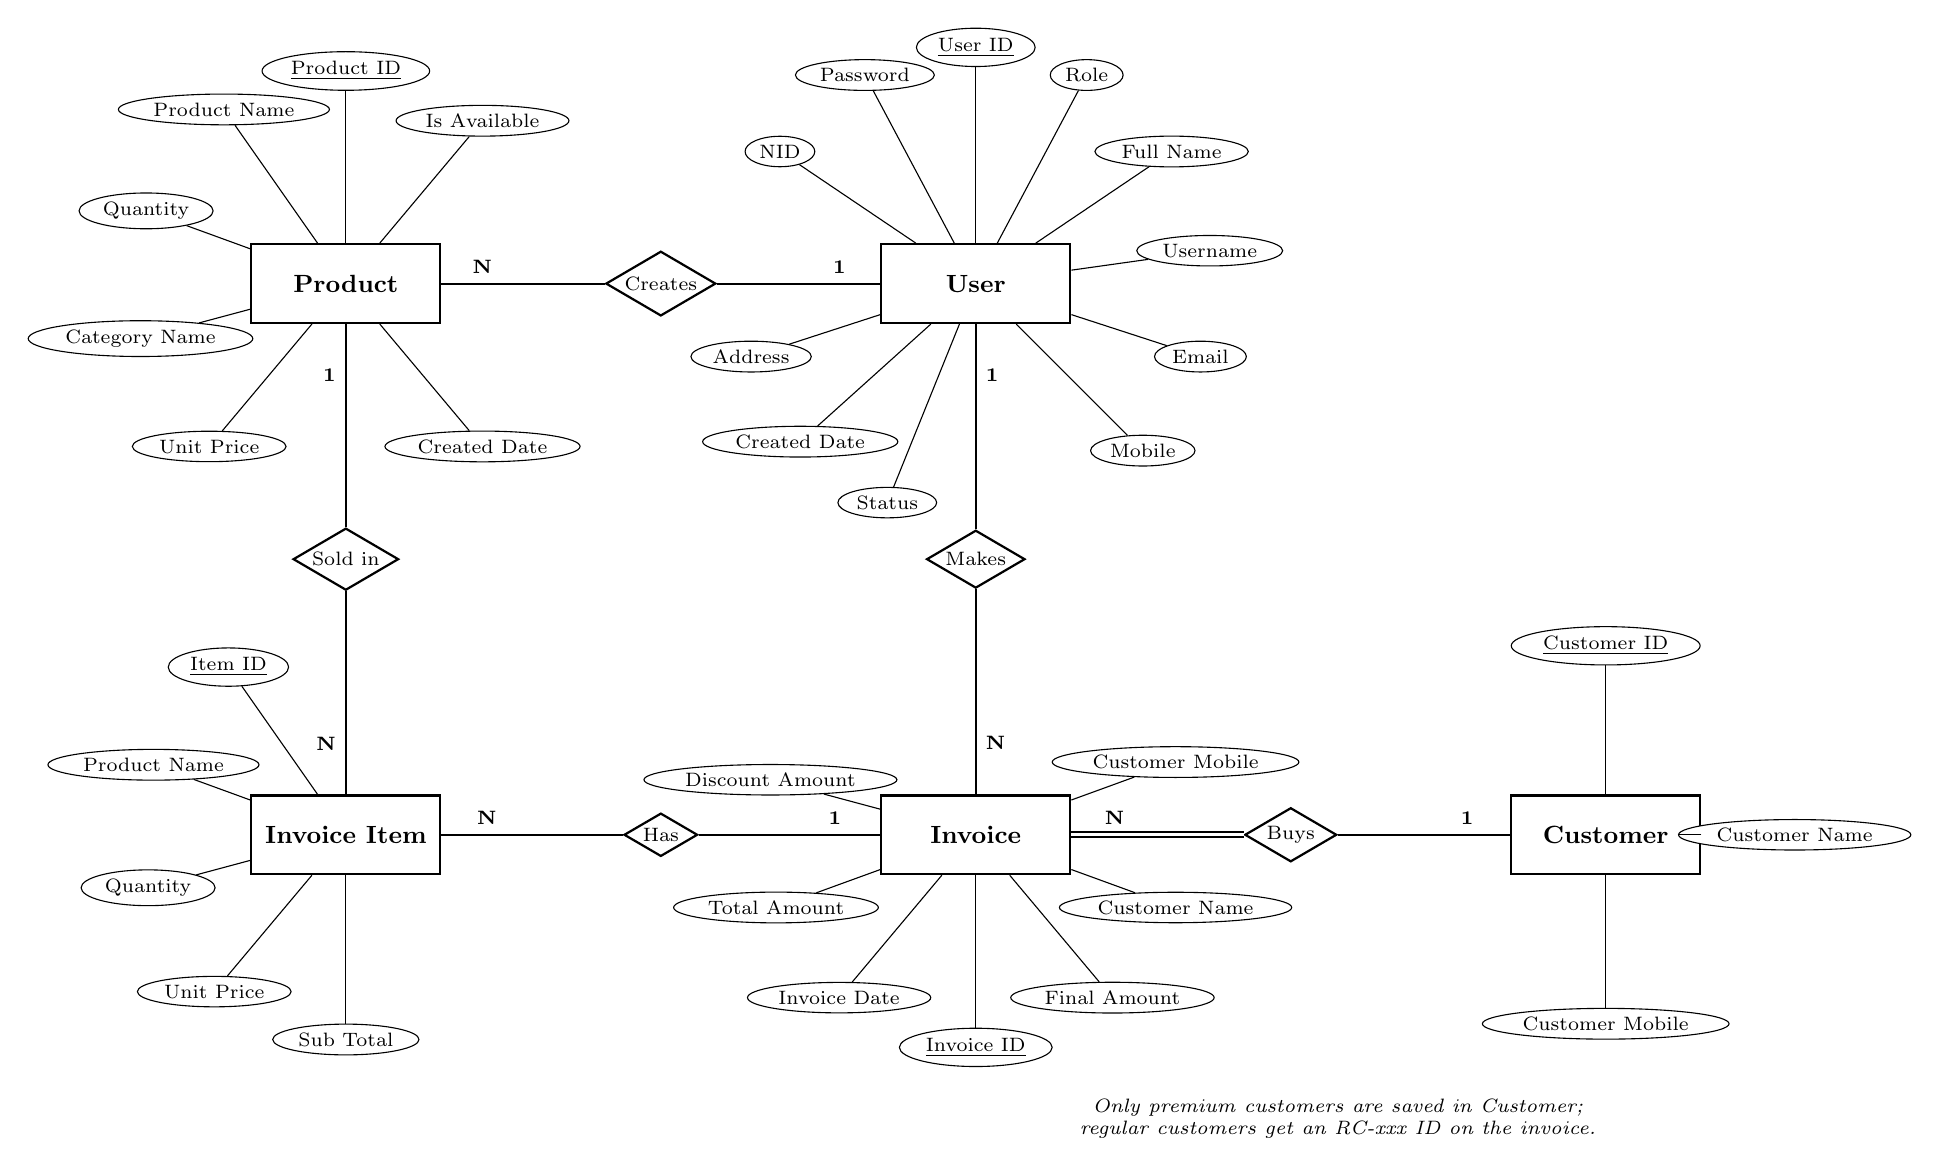
\begin{tikzpicture}[
  font=\footnotesize,
  entity/.style={draw, line width=0.8pt, minimum width=2.4cm, minimum height=1.0cm, font=\small\bfseries, fill=white},
  rel/.style={draw, diamond, aspect=1.7, line width=0.8pt, inner sep=1pt, font=\scriptsize, fill=white, align=center},
  attr/.style={draw, ellipse, inner sep=1.5pt, font=\scriptsize, fill=white},
  card/.style={font=\scriptsize\bfseries}
]
% attributes placed on a circle around an entity: \attrs{entity}{radius}{angle/text,...}
\newcommand{\attrs}[3]{%
  \foreach \a/\t in {#3} {
    \node[attr] (tmp) at ($(#1)+(\a:#2)$) {\t};
    \draw (#1) -- (tmp);
  }}

\usetikzlibrary{calc}

% ---------- entities ----------
\node[entity] (user)     at (0,0)    {User};
\node[entity] (product)  at (-8,0)   {Product};
\node[entity] (invoice)  at (0,-7)   {Invoice};
\node[entity] (item)     at (-8,-7)  {Invoice Item};
\node[entity] (customer) at (8,-7)   {Customer};

% ---------- attributes ----------
\attrs{user}{3.0}{90/\underline{User ID}, 62/Role, 34/Full Name, 8/Username, -18/Email, -45/Mobile, 118/Password, 146/NID, 198/Address, 222/Created Date, 248/Status}
\attrs{product}{2.7}{90/\underline{Product ID}, 125/Product Name, 160/Quantity, 195/Category Name, 230/Unit Price, 310/Created Date, 50/Is Available}
\attrs{invoice}{2.7}{270/\underline{Invoice ID}, 230/Invoice Date, 200/Total Amount, 165/Discount Amount, 310/Final Amount, 340/Customer Name, 20/Customer Mobile}
\attrs{item}{2.6}{125/\underline{Item ID}, 160/Product Name, 195/Quantity, 230/Unit Price, 270/Sub Total}
\attrs{customer}{2.4}{90/\underline{Customer ID}, 0/Customer Name, 270/Customer Mobile}

% ---------- relationships ----------
\node[rel] (creates) at (-4,0)   {Creates};
\node[rel] (makes)   at (0,-3.5) {Makes};
\node[rel] (has)     at (-4,-7)  {Has};
\node[rel] (sold)    at (-8,-3.5){Sold in};
\node[rel] (buys)    at (4,-7)   {Buys};

\draw[line width=0.7pt] (user) -- node[card, above, pos=0.25]{1} (creates) -- node[card, above, pos=0.75]{N} (product);
\draw[line width=0.7pt] (user) -- node[card, right, pos=0.25]{1} (makes) -- node[card, right, pos=0.75]{N} (invoice);
\draw[line width=0.7pt] (invoice) -- node[card, above, pos=0.25]{1} (has) -- node[card, above, pos=0.75]{N} (item);
\draw[line width=0.7pt] (product) -- node[card, left, pos=0.25]{1} (sold) -- node[card, left, pos=0.75]{N} (item);
\draw[line width=0.7pt] (customer) -- node[card, above, pos=0.25]{1} (buys);
\draw[line width=0.7pt, double distance=1.2pt] (buys) -- node[card, above, pos=0.75]{N} (invoice);
\node[font=\scriptsize\itshape, align=center] at (4.6,-10.6) {Only premium customers are saved in Customer;\\regular customers get an RC-xxx ID on the invoice.};
\end{tikzpicture}
\end{document}
